本章专注于能使我们高质量地完成向下延拓波场的技术细节。这章内容很少会有新的地
震成像概念,然而,将有一些关于潜在危险的有趣例子,而且为了改善地层的地震映象之质
量,将要介绍若干新颖有趣的数学概念。本章将近结尾处,备有用以模拟和比较各种偏移方
法的程序。

\subsection{滤波魔术}
\label{sec:4.0.1}

我们在本章内首先要考虑的事情是信号强度。反射是随时间而变弱的,这将影响地震映
象,因而需要进行补偿。

其次,地震资料是受滤波作甩影响的,这种滤波既可在时间域内完成,也可在空间域内完
成。时间序列分析包含有以滤波压制谱的某些频带而增强另外一些频带这种增强信噪比的概
念,也可以在频率$\omega$与波数$k$空间内对波场采取谱加权的办法。当不存在噪音时,波动方程
理论告诉我们应采用什么滤波算子。不大严格地讲,波动方程本身就是一种在$(\omega,k)$空间内
具有平缓振幅响应和相应于传播时间延迟之相位响应的滤波。在$(\omega,k)$空间的不同区域有
不同数量的噪音,但是除了必须按相等比例关系$\Delta x=\Delta z$加以显示,没必要按波动方程所提
供的强度将不同区域全部显示出来。

空间Nyquist频率的性态提供了一个混合应用滤波理论和偏移理论的例子。因为地震数
据总是存在空间假频的,所以这个例子并非没有实际意义。试考虑一种业已消除了
Nyquist
频率的脉冲函数,消除的结果对脉冲本身的有关影响是很小的,可是对该脉冲周围的零点的有
关影响却很巨大。当用频率域方法对一个脉冲进行偏移时,对待低于空间Nyquist频率的
空间频率是非常不同于高于它的频率的,一个是按向左倾对待,另一个则是按右倾对待。在
空间频率域内的这类不连续性形成了一种虚假的、散布很广的空间域响应,如图\ref{fig:dspr/hypnoise}所
示。

\begin{figure}[H]
\centering
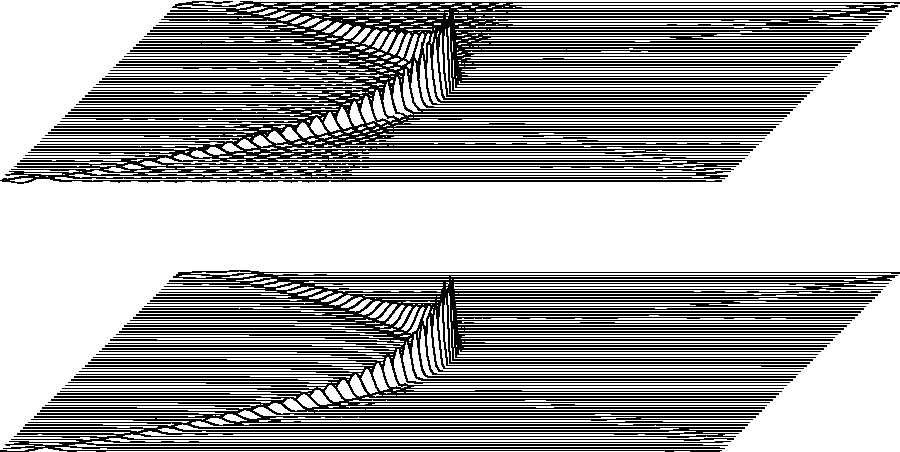
\includegraphics[width=0.65\textwidth]{dspr/hypnoise}
\caption[hypnoise]{表现环绕脉冲的Nyquist噪音,双曲线业已放大(顶部),
及采用滤波方法消除噪音的结果(底部)}
\label{fig:dspr/hypnoise}
\end{figure}

能很容易地压制掉虚假的Nyquist噪音。并不是由于在显示时排除了Nyquist频率,而
只不过是由于采用了一种窄频带滤波,诸如在显示中所采用的滤波、即$
(1+\cos(k_x) \Delta x)/(1+0.85\cos(k_x)\Delta x)$,
这种滤波特性能在空间Nyquist频率上平滑地趋向零点。在横向坐标$x$域内,
这种滤波算子具有一种简单的三对角线表达形式。

\subsection{改善提高偏移技木的展望}
\label{sec:4.0.2}

在我们进行提高质量的'探索追求时,我们也将回顾一下我们正在采用的各秤近似方法。
看一看采用近似如何使结果变坏,并进而发现应如何去改善那些结果,进行这些工作现在该
是时候了。将要考虑的有六个方面的具体问题;
\begin{enumerate}
\item 
以差分算子来近似微分算子时所形成的频散影响;

\item 
因平方根近似而形成的相位与群速度之各向异性畸变;

\item
测线末端的截断效应;

\item
倾角大于$90$度时的影响;

\item
Fourier变换的折叠频率问题;

\item 
速度对Stolt偏移方法的影响以及如何用拉伸的办法改善其结果。

\end{enumerate}


在研究了这些近似影响之后,\ref{sec:4.6}节进而对因果性(causality)\footnote{
有的文献中称作物理可实现性。无论因果性或物理可实现性,均指激发前不应存在响应,波场处于静止状态
的这种性质。---译者
}进行了透彻的研究,
这个问题涉及许多研究课题,包括Fourier频率域偏移方法如何才能模拟时间域偏移所固有
的因果性条件这类问题在内。\ref{sec:4.7}节是总的关于这种多技术的总结,该节提出一种可以根据
许多不同偏移方法来模:拟绕射双曲线的程序,这很方便于比较各种技术和参量的优化。本章
中的图\ref{fig:dspr/hypnoise}与其他许多图件均系用此程序产生,所以你将能够重新产生它们。

\subsection{生产中的潜在危险:$v(x)$形成之弱不稳定性}
\label{sec:3.0.3}

某些质量问题是不可以在Fourier频率域内理解的,除非细心地加以处理,不然速度的
横向变化可以引起不稳定性。

横向的速度跃变形成了陡断层反射。更为严重的问题是:各种外推方程本身始终还未曾
仔细论证过,本书中所包括的各外推方程其最精确的导出方法迄今只是根据波散关系完成
的,而波散关系本身却是意味着沿$x$坐标方向的速度应是恒定的。包含有项的一种波散关
系究竟应该如何表示的问题,还从未得到过答复。也许这可以用$v(x,z)\partial_{xx}$、
$\partial_xv(x,z)\partial_x$、$\partial_{xx}v(x,z)$等项或者它们的任何一种组合来表示,然而,这些表达式的每一种都隐含有数值
彼此不同的内部反射系数。更糟糕的是,到了把所有坐标轴都加以离散化的时候,结果却表
明最为灵敏的一个表示式会导致反射系数大于1,从而导致数值不稳定性。

弱不稳定性比强不稳定性更坏。强不稳定性还能立即引起注意,而弱不稳定性却可能逃
脱人们的注意,从而在以后导致不正确的地球物理结论。幸好,稳定性分析可导出一种在
\ref{sec:4.8}节中将要讨论的防弹法(bullet proof method)。
